\documentclass[twoside]{book}

% Packages required by doxygen
\usepackage{fixltx2e}
\usepackage{calc}
\usepackage{doxygen}
\usepackage[export]{adjustbox} % also loads graphicx
\usepackage{graphicx}
\usepackage[utf8]{inputenc}
\usepackage{makeidx}
\usepackage{multicol}
\usepackage{multirow}
\PassOptionsToPackage{warn}{textcomp}
\usepackage{textcomp}
\usepackage[nointegrals]{wasysym}
\usepackage[table]{xcolor}

% Font selection
\usepackage[T1]{fontenc}
\usepackage[scaled=.90]{helvet}
\usepackage{courier}
\usepackage{amssymb}
\usepackage{sectsty}
\renewcommand{\familydefault}{\sfdefault}
\allsectionsfont{%
  \fontseries{bc}\selectfont%
  \color{darkgray}%
}
\renewcommand{\DoxyLabelFont}{%
  \fontseries{bc}\selectfont%
  \color{darkgray}%
}
\newcommand{\+}{\discretionary{\mbox{\scriptsize$\hookleftarrow$}}{}{}}

% Page & text layout
\usepackage{geometry}
\geometry{%
  a4paper,%
  top=2.5cm,%
  bottom=2.5cm,%
  left=2.5cm,%
  right=2.5cm%
}
\tolerance=750
\hfuzz=15pt
\hbadness=750
\setlength{\emergencystretch}{15pt}
\setlength{\parindent}{0cm}
\setlength{\parskip}{3ex plus 2ex minus 2ex}
\makeatletter
\renewcommand{\paragraph}{%
  \@startsection{paragraph}{4}{0ex}{-1.0ex}{1.0ex}{%
    \normalfont\normalsize\bfseries\SS@parafont%
  }%
}
\renewcommand{\subparagraph}{%
  \@startsection{subparagraph}{5}{0ex}{-1.0ex}{1.0ex}{%
    \normalfont\normalsize\bfseries\SS@subparafont%
  }%
}
\makeatother

% Headers & footers
\usepackage{fancyhdr}
\pagestyle{fancyplain}
\fancyhead[LE]{\fancyplain{}{\bfseries\thepage}}
\fancyhead[CE]{\fancyplain{}{}}
\fancyhead[RE]{\fancyplain{}{\bfseries\leftmark}}
\fancyhead[LO]{\fancyplain{}{\bfseries\rightmark}}
\fancyhead[CO]{\fancyplain{}{}}
\fancyhead[RO]{\fancyplain{}{\bfseries\thepage}}
\fancyfoot[LE]{\fancyplain{}{}}
\fancyfoot[CE]{\fancyplain{}{}}
\fancyfoot[RE]{\fancyplain{}{\bfseries\scriptsize Generated by Doxygen }}
\fancyfoot[LO]{\fancyplain{}{\bfseries\scriptsize Generated by Doxygen }}
\fancyfoot[CO]{\fancyplain{}{}}
\fancyfoot[RO]{\fancyplain{}{}}
\renewcommand{\footrulewidth}{0.4pt}
\renewcommand{\chaptermark}[1]{%
  \markboth{#1}{}%
}
\renewcommand{\sectionmark}[1]{%
  \markright{\thesection\ #1}%
}

% Indices & bibliography
\usepackage{natbib}
\usepackage[titles]{tocloft}
\setcounter{tocdepth}{3}
\setcounter{secnumdepth}{5}
\makeindex

% Hyperlinks (required, but should be loaded last)
\usepackage{ifpdf}
\ifpdf
  \usepackage[pdftex,pagebackref=true]{hyperref}
\else
  \usepackage[ps2pdf,pagebackref=true]{hyperref}
\fi
\hypersetup{%
  colorlinks=true,%
  linkcolor=blue,%
  citecolor=blue,%
  unicode%
}

% Custom commands
\newcommand{\clearemptydoublepage}{%
  \newpage{\pagestyle{empty}\cleardoublepage}%
}

\usepackage{caption}
\captionsetup{labelsep=space,justification=centering,font={bf},singlelinecheck=off,skip=4pt,position=top}

%===== C O N T E N T S =====

\begin{document}

% Titlepage & ToC
\hypersetup{pageanchor=false,
             bookmarksnumbered=true,
             pdfencoding=unicode
            }
\pagenumbering{alph}
\begin{titlepage}
\vspace*{7cm}
\begin{center}%
{\Large X\+N\+LO -\/ U\+P\+PE \\[1ex]\large 1.\+3.\+0 }\\
\vspace*{1cm}
{\large Generated by Doxygen 1.8.13}\\
\end{center}
\end{titlepage}
\clearemptydoublepage
\pagenumbering{roman}
\tableofcontents
\clearemptydoublepage
\pagenumbering{arabic}
\hypersetup{pageanchor=true}

%--- Begin generated contents ---
\chapter{Namespace Index}
\section{Namespace List}
Here is a list of all namespaces with brief descriptions\+:\begin{DoxyCompactList}
\item\contentsline{section}{\mbox{\hyperlink{namespace_h_h}{HH}} }{\pageref{namespace_h_h}}{}
\item\contentsline{section}{\mbox{\hyperlink{namespace_x_n_l_o}{X\+N\+LO}} }{\pageref{namespace_x_n_l_o}}{}
\end{DoxyCompactList}

\chapter{Class Index}
\section{Class List}
Here are the classes, structs, unions and interfaces with brief descriptions\+:\begin{DoxyCompactList}
\item\contentsline{section}{\hyperlink{class_h_h_1_1_config___settings}{H\+H\+::\+Config\+\_\+\+Settings} }{\pageref{class_h_h_1_1_config___settings}}{}
\item\contentsline{section}{\hyperlink{structdetect}{detect$<$ typename, class, typename $>$} }{\pageref{structdetect}}{}
\item\contentsline{section}{\hyperlink{structdetect_3_01_t_00_01_op_00_01void__t_3_01_op_3_01_t_01_4_01_4_01_4}{detect$<$ T, Op, void\+\_\+t$<$ Op$<$ T $>$ $>$ $>$} }{\pageref{structdetect_3_01_t_00_01_op_00_01void__t_3_01_op_3_01_t_01_4_01_4_01_4}}{}
\item\contentsline{section}{\hyperlink{class_d_h_t}{D\+HT} }{\pageref{class_d_h_t}}{}
\item\contentsline{section}{\hyperlink{classgrid__rkr}{grid\+\_\+rkr} }{\pageref{classgrid__rkr}}{}
\item\contentsline{section}{\hyperlink{classgrid__tw}{grid\+\_\+tw} }{\pageref{classgrid__tw}}{}
\item\contentsline{section}{\hyperlink{class_x_n_l_o_1_1grid__tw}{X\+N\+L\+O\+::grid\+\_\+tw} }{\pageref{class_x_n_l_o_1_1grid__tw}}{}
\item\contentsline{section}{\hyperlink{classgrid__xkx}{grid\+\_\+xkx} }{\pageref{classgrid__xkx}}{}
\item\contentsline{section}{\hyperlink{class_h_h__source}{H\+H\+\_\+source} }{\pageref{class_h_h__source}}{}
\item\contentsline{section}{\hyperlink{class_h_h_g_p}{H\+H\+GP} }{\pageref{class_h_h_g_p}}{}
\item\contentsline{section}{\hyperlink{class_i_o}{IO} }{\pageref{class_i_o}}{}
\item\contentsline{section}{\hyperlink{classkeldysh__gas}{keldysh\+\_\+gas} }{\pageref{classkeldysh__gas}}{}
\item\contentsline{section}{\hyperlink{classmaths__textbook}{maths\+\_\+textbook} }{\pageref{classmaths__textbook}}{}
\item\contentsline{section}{\hyperlink{classphysics__textbook}{physics\+\_\+textbook} }{\pageref{classphysics__textbook}}{}
\item\contentsline{section}{\hyperlink{classpropagation}{propagation} }{\pageref{classpropagation}}{}
\end{DoxyCompactList}

\chapter{File Index}
\section{File List}
Here is a list of all files with brief descriptions\+:\begin{DoxyCompactList}
\item\contentsline{section}{/\+Users/sms1n16/\+Project/\+X\+N\+L\+O/src/\+D\+H\+T/\hyperlink{_d_h_t_8cpp}{D\+H\+T.\+cpp} }{\pageref{_d_h_t_8cpp}}{}
\item\contentsline{section}{/\+Users/sms1n16/\+Project/\+X\+N\+L\+O/src/\+D\+H\+T/\hyperlink{_d_h_t_8hpp}{D\+H\+T.\+hpp} }{\pageref{_d_h_t_8hpp}}{}
\item\contentsline{section}{/\+Users/sms1n16/\+Project/\+X\+N\+L\+O/src/gas/\hyperlink{keldysh__gas_8cpp}{keldysh\+\_\+gas.\+cpp} }{\pageref{keldysh__gas_8cpp}}{}
\item\contentsline{section}{/\+Users/sms1n16/\+Project/\+X\+N\+L\+O/src/gas/\hyperlink{keldysh__gas_8hpp}{keldysh\+\_\+gas.\+hpp} }{\pageref{keldysh__gas_8hpp}}{}
\item\contentsline{section}{/\+Users/sms1n16/\+Project/\+X\+N\+L\+O/src/grid/\hyperlink{grid__rkr_8cpp}{grid\+\_\+rkr.\+cpp} }{\pageref{grid__rkr_8cpp}}{}
\item\contentsline{section}{/\+Users/sms1n16/\+Project/\+X\+N\+L\+O/src/grid/\hyperlink{grid__rkr_8hpp}{grid\+\_\+rkr.\+hpp} }{\pageref{grid__rkr_8hpp}}{}
\item\contentsline{section}{/\+Users/sms1n16/\+Project/\+X\+N\+L\+O/src/grid/\hyperlink{grid__tw_8cpp}{grid\+\_\+tw.\+cpp} }{\pageref{grid__tw_8cpp}}{}
\item\contentsline{section}{/\+Users/sms1n16/\+Project/\+X\+N\+L\+O/src/grid/\hyperlink{grid__tw_8hpp}{grid\+\_\+tw.\+hpp} }{\pageref{grid__tw_8hpp}}{}
\item\contentsline{section}{/\+Users/sms1n16/\+Project/\+X\+N\+L\+O/src/grid/\hyperlink{grid__xkx_8cpp}{grid\+\_\+xkx.\+cpp} }{\pageref{grid__xkx_8cpp}}{}
\item\contentsline{section}{/\+Users/sms1n16/\+Project/\+X\+N\+L\+O/src/grid/\hyperlink{grid__xkx_8hpp}{grid\+\_\+xkx.\+hpp} }{\pageref{grid__xkx_8hpp}}{}
\item\contentsline{section}{/\+Users/sms1n16/\+Project/\+X\+N\+L\+O/src/\+H\+H\+G\+P/\hyperlink{config__settings_8cpp}{config\+\_\+settings.\+cpp} }{\pageref{config__settings_8cpp}}{}
\item\contentsline{section}{/\+Users/sms1n16/\+Project/\+X\+N\+L\+O/src/\+H\+H\+G\+P/\hyperlink{config__settings_8hpp}{config\+\_\+settings.\+hpp} }{\pageref{config__settings_8hpp}}{}
\item\contentsline{section}{/\+Users/sms1n16/\+Project/\+X\+N\+L\+O/src/\+H\+H\+G\+P/\hyperlink{_h_h__source_8cpp}{H\+H\+\_\+source.\+cpp} }{\pageref{_h_h__source_8cpp}}{}
\item\contentsline{section}{/\+Users/sms1n16/\+Project/\+X\+N\+L\+O/src/\+H\+H\+G\+P/\hyperlink{_h_h__source_8hpp}{H\+H\+\_\+source.\+hpp} }{\pageref{_h_h__source_8hpp}}{}
\item\contentsline{section}{/\+Users/sms1n16/\+Project/\+X\+N\+L\+O/src/\+H\+H\+G\+P/\hyperlink{_h_h_g_p_8cpp}{H\+H\+G\+P.\+cpp} }{\pageref{_h_h_g_p_8cpp}}{}
\item\contentsline{section}{/\+Users/sms1n16/\+Project/\+X\+N\+L\+O/src/\+H\+H\+G\+P/\hyperlink{_h_h_g_p_8hpp}{H\+H\+G\+P.\+hpp} }{\pageref{_h_h_g_p_8hpp}}{}
\item\contentsline{section}{/\+Users/sms1n16/\+Project/\+X\+N\+L\+O/src/\+H\+H\+G\+P/\hyperlink{main_8cpp}{main.\+cpp} }{\pageref{main_8cpp}}{}
\item\contentsline{section}{/\+Users/sms1n16/\+Project/\+X\+N\+L\+O/src/\+H\+H\+G\+P/\hyperlink{propagation_8cpp}{propagation.\+cpp} }{\pageref{propagation_8cpp}}{}
\item\contentsline{section}{/\+Users/sms1n16/\+Project/\+X\+N\+L\+O/src/\+H\+H\+G\+P/\hyperlink{propagation_8hpp}{propagation.\+hpp} }{\pageref{propagation_8hpp}}{}
\item\contentsline{section}{/\+Users/sms1n16/\+Project/\+X\+N\+L\+O/src/\+I\+O/\hyperlink{_i_o_8cpp}{I\+O.\+cpp} }{\pageref{_i_o_8cpp}}{}
\item\contentsline{section}{/\+Users/sms1n16/\+Project/\+X\+N\+L\+O/src/\+I\+O/\hyperlink{_i_o_8hpp}{I\+O.\+hpp} }{\pageref{_i_o_8hpp}}{}
\item\contentsline{section}{/\+Users/sms1n16/\+Project/\+X\+N\+L\+O/src/maths/\hyperlink{maths__textbook_8cpp}{maths\+\_\+textbook.\+cpp} }{\pageref{maths__textbook_8cpp}}{}
\item\contentsline{section}{/\+Users/sms1n16/\+Project/\+X\+N\+L\+O/src/maths/\hyperlink{maths__textbook_8hpp}{maths\+\_\+textbook.\+hpp} }{\pageref{maths__textbook_8hpp}}{}
\item\contentsline{section}{/\+Users/sms1n16/\+Project/\+X\+N\+L\+O/src/physics/\hyperlink{physics__textbook_8cpp}{physics\+\_\+textbook.\+cpp} }{\pageref{physics__textbook_8cpp}}{}
\item\contentsline{section}{/\+Users/sms1n16/\+Project/\+X\+N\+L\+O/src/physics/\hyperlink{physics__textbook_8hpp}{physics\+\_\+textbook.\+hpp} }{\pageref{physics__textbook_8hpp}}{}
\end{DoxyCompactList}

\chapter{Namespace Documentation}
\input{namespace_h_h}
\chapter{Class Documentation}
\input{class_h_h_1_1_config___settings}
\hypertarget{class_h_h__source}{}\section{H\+H\+\_\+source Class Reference}
\label{class_h_h__source}\index{H\+H\+\_\+source@{H\+H\+\_\+source}}


{\ttfamily \#include $<$H\+H\+\_\+source.\+hpp$>$}



Collaboration diagram for H\+H\+\_\+source\+:\nopagebreak
\begin{figure}[H]
\begin{center}
\leavevmode
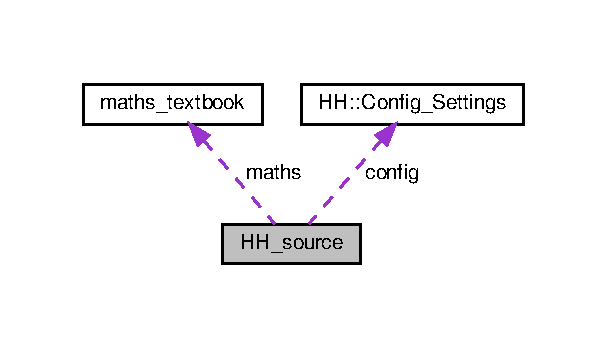
\includegraphics[width=292pt]{class_h_h__source__coll__graph}
\end{center}
\end{figure}
\subsection*{Public Member Functions}
\begin{DoxyCompactItemize}
\item 
\hyperlink{class_h_h__source_a0b3c052d274495b4f90fb09d15fff9fa}{H\+H\+\_\+source} ()
\item 
Array\+X\+Xcd \hyperlink{class_h_h__source_a059c934be1aaa0ed411fea5374bb2428}{Get\+Source} (int \hyperlink{class_h_h__source_a6631481cc1bea05ab564cb1841644a12}{file\+Number}, \hyperlink{class_h_h_1_1_config___settings}{H\+H\+::\+Config\+\_\+\+Settings} \hyperlink{class_h_h__source_adbab95c09c583e2aeebbb4679e6998e8}{config}, \hyperlink{classmaths__textbook}{maths\+\_\+textbook} \hyperlink{class_h_h__source_a93637ad30af846dd04eb741437114f8f}{maths})
\end{DoxyCompactItemize}
\subsection*{Private Attributes}
\begin{DoxyCompactItemize}
\item 
int \hyperlink{class_h_h__source_a6631481cc1bea05ab564cb1841644a12}{file\+Number}
\item 
\hyperlink{class_h_h_1_1_config___settings}{H\+H\+::\+Config\+\_\+\+Settings} \hyperlink{class_h_h__source_adbab95c09c583e2aeebbb4679e6998e8}{config}
\item 
\hyperlink{classmaths__textbook}{maths\+\_\+textbook} \hyperlink{class_h_h__source_a93637ad30af846dd04eb741437114f8f}{maths}
\end{DoxyCompactItemize}


\subsection{Constructor \& Destructor Documentation}
\mbox{\Hypertarget{class_h_h__source_a0b3c052d274495b4f90fb09d15fff9fa}\label{class_h_h__source_a0b3c052d274495b4f90fb09d15fff9fa}} 
\index{H\+H\+\_\+source@{H\+H\+\_\+source}!H\+H\+\_\+source@{H\+H\+\_\+source}}
\index{H\+H\+\_\+source@{H\+H\+\_\+source}!H\+H\+\_\+source@{H\+H\+\_\+source}}
\subsubsection{\texorpdfstring{H\+H\+\_\+source()}{HH\_source()}}
{\footnotesize\ttfamily H\+H\+\_\+source\+::\+H\+H\+\_\+source (\begin{DoxyParamCaption}{ }\end{DoxyParamCaption})}



\subsection{Member Function Documentation}
\mbox{\Hypertarget{class_h_h__source_a059c934be1aaa0ed411fea5374bb2428}\label{class_h_h__source_a059c934be1aaa0ed411fea5374bb2428}} 
\index{H\+H\+\_\+source@{H\+H\+\_\+source}!Get\+Source@{Get\+Source}}
\index{Get\+Source@{Get\+Source}!H\+H\+\_\+source@{H\+H\+\_\+source}}
\subsubsection{\texorpdfstring{Get\+Source()}{GetSource()}}
{\footnotesize\ttfamily Array\+X\+Xcd H\+H\+\_\+source\+::\+Get\+Source (\begin{DoxyParamCaption}\item[{int}]{file\+Number,  }\item[{\hyperlink{class_h_h_1_1_config___settings}{H\+H\+::\+Config\+\_\+\+Settings}}]{config,  }\item[{\hyperlink{classmaths__textbook}{maths\+\_\+textbook}}]{maths }\end{DoxyParamCaption})}



\subsection{Member Data Documentation}
\mbox{\Hypertarget{class_h_h__source_adbab95c09c583e2aeebbb4679e6998e8}\label{class_h_h__source_adbab95c09c583e2aeebbb4679e6998e8}} 
\index{H\+H\+\_\+source@{H\+H\+\_\+source}!config@{config}}
\index{config@{config}!H\+H\+\_\+source@{H\+H\+\_\+source}}
\subsubsection{\texorpdfstring{config}{config}}
{\footnotesize\ttfamily \hyperlink{class_h_h_1_1_config___settings}{H\+H\+::\+Config\+\_\+\+Settings} H\+H\+\_\+source\+::config\hspace{0.3cm}{\ttfamily [private]}}

\mbox{\Hypertarget{class_h_h__source_a6631481cc1bea05ab564cb1841644a12}\label{class_h_h__source_a6631481cc1bea05ab564cb1841644a12}} 
\index{H\+H\+\_\+source@{H\+H\+\_\+source}!file\+Number@{file\+Number}}
\index{file\+Number@{file\+Number}!H\+H\+\_\+source@{H\+H\+\_\+source}}
\subsubsection{\texorpdfstring{file\+Number}{fileNumber}}
{\footnotesize\ttfamily int H\+H\+\_\+source\+::file\+Number\hspace{0.3cm}{\ttfamily [private]}}

\mbox{\Hypertarget{class_h_h__source_a93637ad30af846dd04eb741437114f8f}\label{class_h_h__source_a93637ad30af846dd04eb741437114f8f}} 
\index{H\+H\+\_\+source@{H\+H\+\_\+source}!maths@{maths}}
\index{maths@{maths}!H\+H\+\_\+source@{H\+H\+\_\+source}}
\subsubsection{\texorpdfstring{maths}{maths}}
{\footnotesize\ttfamily \hyperlink{classmaths__textbook}{maths\+\_\+textbook} H\+H\+\_\+source\+::maths\hspace{0.3cm}{\ttfamily [private]}}



The documentation for this class was generated from the following files\+:\begin{DoxyCompactItemize}
\item 
/\+Users/sms1n16/\+Project/\+X\+N\+L\+O/src/\+H\+H\+G\+P/\hyperlink{_h_h__source_8hpp}{H\+H\+\_\+source.\+hpp}\item 
/\+Users/sms1n16/\+Project/\+X\+N\+L\+O/src/\+H\+H\+G\+P/\hyperlink{_h_h__source_8cpp}{H\+H\+\_\+source.\+cpp}\end{DoxyCompactItemize}

\input{class_h_h_g_p}
\hypertarget{classpropagation}{}\section{propagation Class Reference}
\label{classpropagation}\index{propagation@{propagation}}


{\ttfamily \#include $<$propagation.\+hpp$>$}



Collaboration diagram for propagation\+:\nopagebreak
\begin{figure}[H]
\begin{center}
\leavevmode
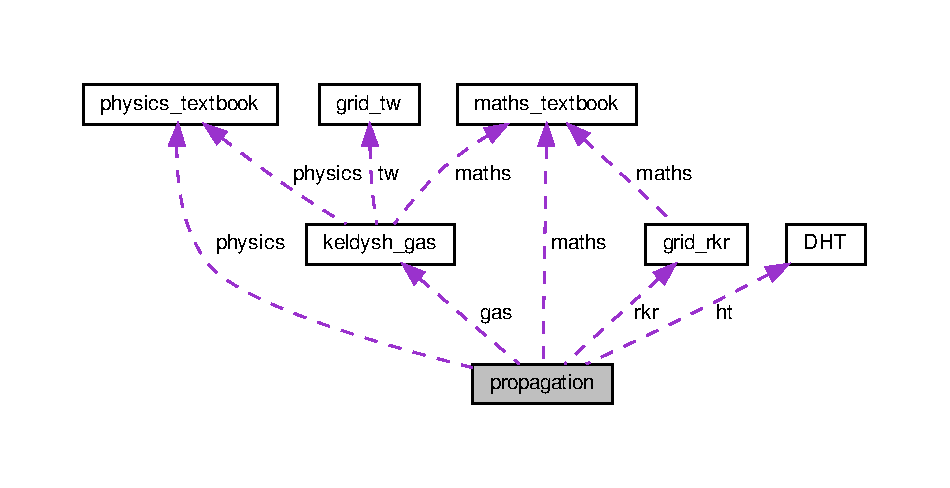
\includegraphics[width=345pt]{classpropagation__coll__graph}
\end{center}
\end{figure}
\subsection*{Public Member Functions}
\begin{DoxyCompactItemize}
\item 
\hyperlink{classpropagation_a9d7b9f42ce1c0bc741d3016a07ba13f7}{propagation} ()
\item 
\hyperlink{classpropagation_ab815c7ad4d93eaa7b7b821908fdc3203}{propagation} (double E\+\_\+min\+\_\+, Eigen\+::\+Array\+Xd w\+\_\+active\+\_\+, \hyperlink{classkeldysh__gas}{keldysh\+\_\+gas} \&gas\+\_\+, grid\+\_\+rkr \&rkr\+\_\+, \hyperlink{classphysics__textbook}{physics\+\_\+textbook} \&physics\+\_\+, \hyperlink{classmaths__textbook}{maths\+\_\+textbook} \&maths\+\_\+, D\+HT \&ht\+\_\+)
\item 
Eigen\+::\+Array\+Xd \hyperlink{classpropagation_a39126bbbd4977c140c0077b849e78bc1}{segment} (Eigen\+::\+Array\+Xd \hyperlink{classpropagation_a49a30e941421cd5e3f0b62bd1335a767}{k})
\item 
Eigen\+::\+Array\+X\+Xcd \hyperlink{classpropagation_af12b15d9b91f98516c0ff25efc1233d1}{block} (Eigen\+::\+Array\+X\+Xcd A\+\_\+w\+\_\+e\+\_\+)
\item 
std\+::complex$<$ double $>$ \hyperlink{classpropagation_a7c696d9e54e5f0a7735047e28aee4866}{n} (int i)
\item 
void \hyperlink{classpropagation_a65e272beb6b5b73f433456361bcde914}{near\+Field\+Propagation\+Step} (double dz, Eigen\+::\+Array\+X\+Xcd A\+\_\+w\+\_\+r\+\_\+)
\item 
void \hyperlink{classpropagation_a9c2e1cb4e314c173b26de08ffcfe071d}{far\+Field\+Propagation} ()
\end{DoxyCompactItemize}
\subsection*{Public Attributes}
\begin{DoxyCompactItemize}
\item 
double \hyperlink{classpropagation_aeacfc091fafd1fdb1af4536f6f587e55}{z}
\item 
int \hyperlink{classpropagation_a93033ee98c04a6fe007eae5c856e76b3}{n\+\_\+k}
\item 
Eigen\+::\+Array\+Xd \hyperlink{classpropagation_a4c24f42d4148eded469c6479d6bf1661}{w\+\_\+active}
\item 
Eigen\+::\+Array\+Xcd \hyperlink{classpropagation_a9e437271e452fa1732f50e006347b501}{k\+\_\+r}
\item 
Eigen\+::\+Array\+X\+Xcd \hyperlink{classpropagation_ad3a84addde67e43bbb606408193f78ee}{A\+\_\+w\+\_\+r}
\end{DoxyCompactItemize}
\subsection*{Private Attributes}
\begin{DoxyCompactItemize}
\item 
double \hyperlink{classpropagation_ab5a753d760a135806a93b9082e8019fb}{E\+\_\+min}
\item 
\hyperlink{classphysics__textbook}{physics\+\_\+textbook} \hyperlink{classpropagation_a42a6e725e3dd53cf94192bf93c31c8de}{physics}
\item 
\hyperlink{classmaths__textbook}{maths\+\_\+textbook} \hyperlink{classpropagation_ab5a5024c2d06c0dad06c745af7c6416c}{maths}
\item 
\hyperlink{classkeldysh__gas}{keldysh\+\_\+gas} \hyperlink{classpropagation_a4152dc9a226a7ff91aff2338d0bd813f}{gas}
\item 
grid\+\_\+rkr \hyperlink{classpropagation_a3d37531bb5918f972544d242aec7e72b}{rkr}
\item 
D\+HT \hyperlink{classpropagation_a044544975e7fc2ec3df9a55d92f8cc90}{ht}
\item 
Eigen\+::\+Array\+Xd \hyperlink{classpropagation_a07a80b67a345e3e9d8e934d2265ba288}{w\+\_\+active\+\_\+tmp}
\item 
int \hyperlink{classpropagation_a76f3651eac23a69c1259dc0406fbe0d9}{k\+\_\+excluded}
\item 
Eigen\+::\+Array\+Xcd \hyperlink{classpropagation_a49a30e941421cd5e3f0b62bd1335a767}{k}
\item 
Eigen\+::\+Array\+Xcd \hyperlink{classpropagation_aba601a0df3c63b13215c55d8ade2bcd7}{refractive\+Index}
\item 
Eigen\+::\+Array\+Xcd \hyperlink{classpropagation_a5ae0154dc8db04188ba92e10ba981000}{lamda}
\item 
Eigen\+::\+Array\+Xcd \hyperlink{classpropagation_a4df23dd19a8cca8a4cb032718dc2b258}{A\+\_\+w\+\_\+kr}
\item 
std\+::string \hyperlink{classpropagation_abd78bf6976f2b2d0a3fc82b9cf0d9dc6}{E\+\_\+f1\+\_\+f2\+\_\+data\+\_\+path}
\item 
Eigen\+::\+Array\+X\+Xd \hyperlink{classpropagation_a53ab4838e0e66b55c2ab1398389a22f5}{E\+\_\+f1\+\_\+f2\+\_\+data}
\item 
Eigen\+::\+Array\+Xd \hyperlink{classpropagation_aff3713e9170542e31c952a2d1b760eec}{E}
\item 
Eigen\+::\+Array\+Xd \hyperlink{classpropagation_a747dcaf8f7405a17af992bae39b7fab5}{f2}
\item 
Eigen\+::\+Array\+Xd \hyperlink{classpropagation_a14d6e72396c1c354c6d9986f2d79f85f}{f1}
\end{DoxyCompactItemize}


\subsection{Constructor \& Destructor Documentation}
\mbox{\Hypertarget{classpropagation_a9d7b9f42ce1c0bc741d3016a07ba13f7}\label{classpropagation_a9d7b9f42ce1c0bc741d3016a07ba13f7}} 
\index{propagation@{propagation}!propagation@{propagation}}
\index{propagation@{propagation}!propagation@{propagation}}
\subsubsection{\texorpdfstring{propagation()}{propagation()}\hspace{0.1cm}{\footnotesize\ttfamily [1/2]}}
{\footnotesize\ttfamily propagation\+::propagation (\begin{DoxyParamCaption}{ }\end{DoxyParamCaption})}

Constructor \mbox{\Hypertarget{classpropagation_ab815c7ad4d93eaa7b7b821908fdc3203}\label{classpropagation_ab815c7ad4d93eaa7b7b821908fdc3203}} 
\index{propagation@{propagation}!propagation@{propagation}}
\index{propagation@{propagation}!propagation@{propagation}}
\subsubsection{\texorpdfstring{propagation()}{propagation()}\hspace{0.1cm}{\footnotesize\ttfamily [2/2]}}
{\footnotesize\ttfamily propagation\+::propagation (\begin{DoxyParamCaption}\item[{double}]{E\+\_\+min\+\_\+,  }\item[{Eigen\+::\+Array\+Xd}]{w\+\_\+active\+\_\+,  }\item[{\hyperlink{classkeldysh__gas}{keldysh\+\_\+gas} \&}]{gas\+\_\+,  }\item[{grid\+\_\+rkr \&}]{rkr\+\_\+,  }\item[{\hyperlink{classphysics__textbook}{physics\+\_\+textbook} \&}]{physics\+\_\+,  }\item[{\hyperlink{classmaths__textbook}{maths\+\_\+textbook} \&}]{maths\+\_\+,  }\item[{D\+HT \&}]{ht\+\_\+ }\end{DoxyParamCaption})}



\subsection{Member Function Documentation}
\mbox{\Hypertarget{classpropagation_af12b15d9b91f98516c0ff25efc1233d1}\label{classpropagation_af12b15d9b91f98516c0ff25efc1233d1}} 
\index{propagation@{propagation}!block@{block}}
\index{block@{block}!propagation@{propagation}}
\subsubsection{\texorpdfstring{block()}{block()}}
{\footnotesize\ttfamily Eigen\+::\+Array\+X\+Xcd propagation\+::block (\begin{DoxyParamCaption}\item[{Eigen\+::\+Array\+X\+Xcd}]{A\+\_\+w\+\_\+e\+\_\+ }\end{DoxyParamCaption})}

\mbox{\Hypertarget{classpropagation_a9c2e1cb4e314c173b26de08ffcfe071d}\label{classpropagation_a9c2e1cb4e314c173b26de08ffcfe071d}} 
\index{propagation@{propagation}!far\+Field\+Propagation@{far\+Field\+Propagation}}
\index{far\+Field\+Propagation@{far\+Field\+Propagation}!propagation@{propagation}}
\subsubsection{\texorpdfstring{far\+Field\+Propagation()}{farFieldPropagation()}}
{\footnotesize\ttfamily void propagation\+::far\+Field\+Propagation (\begin{DoxyParamCaption}{ }\end{DoxyParamCaption})}

Fraunhofer diffraction for propagating into the far-\/field. \mbox{\Hypertarget{classpropagation_a7c696d9e54e5f0a7735047e28aee4866}\label{classpropagation_a7c696d9e54e5f0a7735047e28aee4866}} 
\index{propagation@{propagation}!n@{n}}
\index{n@{n}!propagation@{propagation}}
\subsubsection{\texorpdfstring{n()}{n()}}
{\footnotesize\ttfamily std\+::complex$<$ double $>$ propagation\+::n (\begin{DoxyParamCaption}\item[{int}]{i }\end{DoxyParamCaption})}

\mbox{\Hypertarget{classpropagation_a65e272beb6b5b73f433456361bcde914}\label{classpropagation_a65e272beb6b5b73f433456361bcde914}} 
\index{propagation@{propagation}!near\+Field\+Propagation\+Step@{near\+Field\+Propagation\+Step}}
\index{near\+Field\+Propagation\+Step@{near\+Field\+Propagation\+Step}!propagation@{propagation}}
\subsubsection{\texorpdfstring{near\+Field\+Propagation\+Step()}{nearFieldPropagationStep()}}
{\footnotesize\ttfamily void propagation\+::near\+Field\+Propagation\+Step (\begin{DoxyParamCaption}\item[{double}]{dz,  }\item[{Eigen\+::\+Array\+X\+Xcd}]{A\+\_\+w\+\_\+r\+\_\+ }\end{DoxyParamCaption})}

Angular Spectrum Method (A\+SM) for propagating in the near-\/field, in the gas-\/filled capillary. \mbox{[}Need to add citation!\mbox{]} For circularly-\/symmetric geometry\+: \[ E(z, r) = \mathcal{H}^{-1}\left(\mathcal{H}(E(0, r)) \times \exp(iz\sqrt{k^2 - k_r^2})\right). \] \mbox{\Hypertarget{classpropagation_a39126bbbd4977c140c0077b849e78bc1}\label{classpropagation_a39126bbbd4977c140c0077b849e78bc1}} 
\index{propagation@{propagation}!segment@{segment}}
\index{segment@{segment}!propagation@{propagation}}
\subsubsection{\texorpdfstring{segment()}{segment()}}
{\footnotesize\ttfamily Eigen\+::\+Array\+Xd propagation\+::segment (\begin{DoxyParamCaption}\item[{Eigen\+::\+Array\+Xd}]{k }\end{DoxyParamCaption})}



\subsection{Member Data Documentation}
\mbox{\Hypertarget{classpropagation_a4df23dd19a8cca8a4cb032718dc2b258}\label{classpropagation_a4df23dd19a8cca8a4cb032718dc2b258}} 
\index{propagation@{propagation}!A\+\_\+w\+\_\+kr@{A\+\_\+w\+\_\+kr}}
\index{A\+\_\+w\+\_\+kr@{A\+\_\+w\+\_\+kr}!propagation@{propagation}}
\subsubsection{\texorpdfstring{A\+\_\+w\+\_\+kr}{A\_w\_kr}}
{\footnotesize\ttfamily Eigen\+::\+Array\+Xcd propagation\+::\+A\+\_\+w\+\_\+kr\hspace{0.3cm}{\ttfamily [private]}}

\mbox{\Hypertarget{classpropagation_ad3a84addde67e43bbb606408193f78ee}\label{classpropagation_ad3a84addde67e43bbb606408193f78ee}} 
\index{propagation@{propagation}!A\+\_\+w\+\_\+r@{A\+\_\+w\+\_\+r}}
\index{A\+\_\+w\+\_\+r@{A\+\_\+w\+\_\+r}!propagation@{propagation}}
\subsubsection{\texorpdfstring{A\+\_\+w\+\_\+r}{A\_w\_r}}
{\footnotesize\ttfamily Eigen\+::\+Array\+X\+Xcd propagation\+::\+A\+\_\+w\+\_\+r}

\mbox{\Hypertarget{classpropagation_aff3713e9170542e31c952a2d1b760eec}\label{classpropagation_aff3713e9170542e31c952a2d1b760eec}} 
\index{propagation@{propagation}!E@{E}}
\index{E@{E}!propagation@{propagation}}
\subsubsection{\texorpdfstring{E}{E}}
{\footnotesize\ttfamily Eigen\+::\+Array\+Xd propagation\+::E\hspace{0.3cm}{\ttfamily [private]}}

\mbox{\Hypertarget{classpropagation_a53ab4838e0e66b55c2ab1398389a22f5}\label{classpropagation_a53ab4838e0e66b55c2ab1398389a22f5}} 
\index{propagation@{propagation}!E\+\_\+f1\+\_\+f2\+\_\+data@{E\+\_\+f1\+\_\+f2\+\_\+data}}
\index{E\+\_\+f1\+\_\+f2\+\_\+data@{E\+\_\+f1\+\_\+f2\+\_\+data}!propagation@{propagation}}
\subsubsection{\texorpdfstring{E\+\_\+f1\+\_\+f2\+\_\+data}{E\_f1\_f2\_data}}
{\footnotesize\ttfamily Eigen\+::\+Array\+X\+Xd propagation\+::\+E\+\_\+f1\+\_\+f2\+\_\+data\hspace{0.3cm}{\ttfamily [private]}}

\mbox{\Hypertarget{classpropagation_abd78bf6976f2b2d0a3fc82b9cf0d9dc6}\label{classpropagation_abd78bf6976f2b2d0a3fc82b9cf0d9dc6}} 
\index{propagation@{propagation}!E\+\_\+f1\+\_\+f2\+\_\+data\+\_\+path@{E\+\_\+f1\+\_\+f2\+\_\+data\+\_\+path}}
\index{E\+\_\+f1\+\_\+f2\+\_\+data\+\_\+path@{E\+\_\+f1\+\_\+f2\+\_\+data\+\_\+path}!propagation@{propagation}}
\subsubsection{\texorpdfstring{E\+\_\+f1\+\_\+f2\+\_\+data\+\_\+path}{E\_f1\_f2\_data\_path}}
{\footnotesize\ttfamily std\+::string propagation\+::\+E\+\_\+f1\+\_\+f2\+\_\+data\+\_\+path\hspace{0.3cm}{\ttfamily [private]}}

\mbox{\Hypertarget{classpropagation_ab5a753d760a135806a93b9082e8019fb}\label{classpropagation_ab5a753d760a135806a93b9082e8019fb}} 
\index{propagation@{propagation}!E\+\_\+min@{E\+\_\+min}}
\index{E\+\_\+min@{E\+\_\+min}!propagation@{propagation}}
\subsubsection{\texorpdfstring{E\+\_\+min}{E\_min}}
{\footnotesize\ttfamily double propagation\+::\+E\+\_\+min\hspace{0.3cm}{\ttfamily [private]}}

\mbox{\Hypertarget{classpropagation_a14d6e72396c1c354c6d9986f2d79f85f}\label{classpropagation_a14d6e72396c1c354c6d9986f2d79f85f}} 
\index{propagation@{propagation}!f1@{f1}}
\index{f1@{f1}!propagation@{propagation}}
\subsubsection{\texorpdfstring{f1}{f1}}
{\footnotesize\ttfamily Eigen\+::\+Array\+Xd propagation\+::f1\hspace{0.3cm}{\ttfamily [private]}}

\mbox{\Hypertarget{classpropagation_a747dcaf8f7405a17af992bae39b7fab5}\label{classpropagation_a747dcaf8f7405a17af992bae39b7fab5}} 
\index{propagation@{propagation}!f2@{f2}}
\index{f2@{f2}!propagation@{propagation}}
\subsubsection{\texorpdfstring{f2}{f2}}
{\footnotesize\ttfamily Eigen\+::\+Array\+Xd propagation\+::f2\hspace{0.3cm}{\ttfamily [private]}}

\mbox{\Hypertarget{classpropagation_a4152dc9a226a7ff91aff2338d0bd813f}\label{classpropagation_a4152dc9a226a7ff91aff2338d0bd813f}} 
\index{propagation@{propagation}!gas@{gas}}
\index{gas@{gas}!propagation@{propagation}}
\subsubsection{\texorpdfstring{gas}{gas}}
{\footnotesize\ttfamily \hyperlink{classkeldysh__gas}{keldysh\+\_\+gas} propagation\+::gas\hspace{0.3cm}{\ttfamily [private]}}

\mbox{\Hypertarget{classpropagation_a044544975e7fc2ec3df9a55d92f8cc90}\label{classpropagation_a044544975e7fc2ec3df9a55d92f8cc90}} 
\index{propagation@{propagation}!ht@{ht}}
\index{ht@{ht}!propagation@{propagation}}
\subsubsection{\texorpdfstring{ht}{ht}}
{\footnotesize\ttfamily D\+HT propagation\+::ht\hspace{0.3cm}{\ttfamily [private]}}

Hankel transform \mbox{\Hypertarget{classpropagation_a49a30e941421cd5e3f0b62bd1335a767}\label{classpropagation_a49a30e941421cd5e3f0b62bd1335a767}} 
\index{propagation@{propagation}!k@{k}}
\index{k@{k}!propagation@{propagation}}
\subsubsection{\texorpdfstring{k}{k}}
{\footnotesize\ttfamily Eigen\+::\+Array\+Xcd propagation\+::k\hspace{0.3cm}{\ttfamily [private]}}

\mbox{\Hypertarget{classpropagation_a76f3651eac23a69c1259dc0406fbe0d9}\label{classpropagation_a76f3651eac23a69c1259dc0406fbe0d9}} 
\index{propagation@{propagation}!k\+\_\+excluded@{k\+\_\+excluded}}
\index{k\+\_\+excluded@{k\+\_\+excluded}!propagation@{propagation}}
\subsubsection{\texorpdfstring{k\+\_\+excluded}{k\_excluded}}
{\footnotesize\ttfamily int propagation\+::k\+\_\+excluded\hspace{0.3cm}{\ttfamily [private]}}

\mbox{\Hypertarget{classpropagation_a9e437271e452fa1732f50e006347b501}\label{classpropagation_a9e437271e452fa1732f50e006347b501}} 
\index{propagation@{propagation}!k\+\_\+r@{k\+\_\+r}}
\index{k\+\_\+r@{k\+\_\+r}!propagation@{propagation}}
\subsubsection{\texorpdfstring{k\+\_\+r}{k\_r}}
{\footnotesize\ttfamily Eigen\+::\+Array\+Xcd propagation\+::k\+\_\+r}

\mbox{\Hypertarget{classpropagation_a5ae0154dc8db04188ba92e10ba981000}\label{classpropagation_a5ae0154dc8db04188ba92e10ba981000}} 
\index{propagation@{propagation}!lamda@{lamda}}
\index{lamda@{lamda}!propagation@{propagation}}
\subsubsection{\texorpdfstring{lamda}{lamda}}
{\footnotesize\ttfamily Eigen\+::\+Array\+Xcd propagation\+::lamda\hspace{0.3cm}{\ttfamily [private]}}

\mbox{\Hypertarget{classpropagation_ab5a5024c2d06c0dad06c745af7c6416c}\label{classpropagation_ab5a5024c2d06c0dad06c745af7c6416c}} 
\index{propagation@{propagation}!maths@{maths}}
\index{maths@{maths}!propagation@{propagation}}
\subsubsection{\texorpdfstring{maths}{maths}}
{\footnotesize\ttfamily \hyperlink{classmaths__textbook}{maths\+\_\+textbook} propagation\+::maths\hspace{0.3cm}{\ttfamily [private]}}

Mathematical constants and functions \mbox{\Hypertarget{classpropagation_a93033ee98c04a6fe007eae5c856e76b3}\label{classpropagation_a93033ee98c04a6fe007eae5c856e76b3}} 
\index{propagation@{propagation}!n\+\_\+k@{n\+\_\+k}}
\index{n\+\_\+k@{n\+\_\+k}!propagation@{propagation}}
\subsubsection{\texorpdfstring{n\+\_\+k}{n\_k}}
{\footnotesize\ttfamily int propagation\+::n\+\_\+k}

\mbox{\Hypertarget{classpropagation_a42a6e725e3dd53cf94192bf93c31c8de}\label{classpropagation_a42a6e725e3dd53cf94192bf93c31c8de}} 
\index{propagation@{propagation}!physics@{physics}}
\index{physics@{physics}!propagation@{propagation}}
\subsubsection{\texorpdfstring{physics}{physics}}
{\footnotesize\ttfamily \hyperlink{classphysics__textbook}{physics\+\_\+textbook} propagation\+::physics\hspace{0.3cm}{\ttfamily [private]}}

Physical constants \mbox{\Hypertarget{classpropagation_aba601a0df3c63b13215c55d8ade2bcd7}\label{classpropagation_aba601a0df3c63b13215c55d8ade2bcd7}} 
\index{propagation@{propagation}!refractive\+Index@{refractive\+Index}}
\index{refractive\+Index@{refractive\+Index}!propagation@{propagation}}
\subsubsection{\texorpdfstring{refractive\+Index}{refractiveIndex}}
{\footnotesize\ttfamily Eigen\+::\+Array\+Xcd propagation\+::refractive\+Index\hspace{0.3cm}{\ttfamily [private]}}

\mbox{\Hypertarget{classpropagation_a3d37531bb5918f972544d242aec7e72b}\label{classpropagation_a3d37531bb5918f972544d242aec7e72b}} 
\index{propagation@{propagation}!rkr@{rkr}}
\index{rkr@{rkr}!propagation@{propagation}}
\subsubsection{\texorpdfstring{rkr}{rkr}}
{\footnotesize\ttfamily grid\+\_\+rkr propagation\+::rkr\hspace{0.3cm}{\ttfamily [private]}}

Radial grid \mbox{\Hypertarget{classpropagation_a4c24f42d4148eded469c6479d6bf1661}\label{classpropagation_a4c24f42d4148eded469c6479d6bf1661}} 
\index{propagation@{propagation}!w\+\_\+active@{w\+\_\+active}}
\index{w\+\_\+active@{w\+\_\+active}!propagation@{propagation}}
\subsubsection{\texorpdfstring{w\+\_\+active}{w\_active}}
{\footnotesize\ttfamily Eigen\+::\+Array\+Xd propagation\+::w\+\_\+active}

\mbox{\Hypertarget{classpropagation_a07a80b67a345e3e9d8e934d2265ba288}\label{classpropagation_a07a80b67a345e3e9d8e934d2265ba288}} 
\index{propagation@{propagation}!w\+\_\+active\+\_\+tmp@{w\+\_\+active\+\_\+tmp}}
\index{w\+\_\+active\+\_\+tmp@{w\+\_\+active\+\_\+tmp}!propagation@{propagation}}
\subsubsection{\texorpdfstring{w\+\_\+active\+\_\+tmp}{w\_active\_tmp}}
{\footnotesize\ttfamily Eigen\+::\+Array\+Xd propagation\+::w\+\_\+active\+\_\+tmp\hspace{0.3cm}{\ttfamily [private]}}

\mbox{\Hypertarget{classpropagation_aeacfc091fafd1fdb1af4536f6f587e55}\label{classpropagation_aeacfc091fafd1fdb1af4536f6f587e55}} 
\index{propagation@{propagation}!z@{z}}
\index{z@{z}!propagation@{propagation}}
\subsubsection{\texorpdfstring{z}{z}}
{\footnotesize\ttfamily double propagation\+::z}



The documentation for this class was generated from the following files\+:\begin{DoxyCompactItemize}
\item 
/home/sam/\+Project/\+X\+N\+L\+O/\+H\+H\+G\+P/src/\hyperlink{propagation_8hpp}{propagation.\+hpp}\item 
/home/sam/\+Project/\+X\+N\+L\+O/\+H\+H\+G\+P/src/\hyperlink{propagation_8cpp}{propagation.\+cpp}\end{DoxyCompactItemize}

\chapter{File Documentation}
\hypertarget{config__settings_8cpp}{}\section{/\+Users/sms1n16/\+Project/\+X\+N\+L\+O/src/\+H\+H\+G\+P/config\+\_\+settings.cpp File Reference}
\label{config__settings_8cpp}\index{/\+Users/sms1n16/\+Project/\+X\+N\+L\+O/src/\+H\+H\+G\+P/config\+\_\+settings.\+cpp@{/\+Users/sms1n16/\+Project/\+X\+N\+L\+O/src/\+H\+H\+G\+P/config\+\_\+settings.\+cpp}}
{\ttfamily \#include \char`\"{}config\+\_\+settings.\+hpp\char`\"{}}\newline
{\ttfamily \#include $<$fstream$>$}\newline
{\ttfamily \#include $<$iostream$>$}\newline
{\ttfamily \#include $<$string$>$}\newline
Include dependency graph for config\+\_\+settings.\+cpp\+:\nopagebreak
\begin{figure}[H]
\begin{center}
\leavevmode
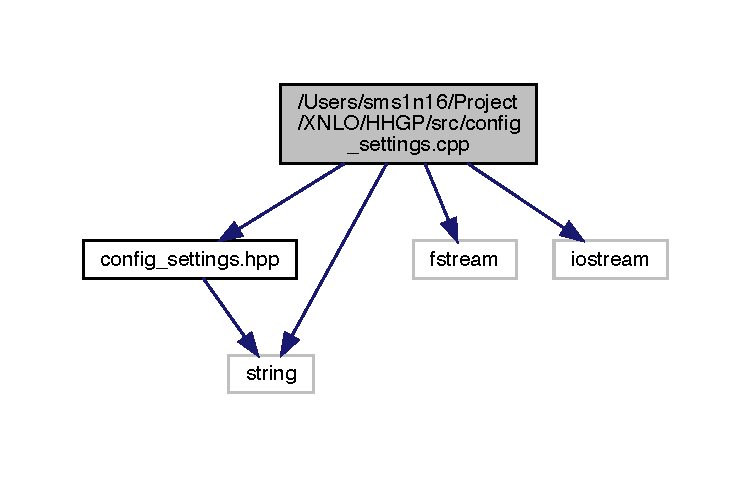
\includegraphics[width=350pt]{config__settings_8cpp__incl}
\end{center}
\end{figure}
\subsection*{Namespaces}
\begin{DoxyCompactItemize}
\item 
 \hyperlink{namespace_h_h}{HH}
\end{DoxyCompactItemize}

\hypertarget{config__settings_8hpp}{}\section{/\+Users/sms1n16/\+Project/\+X\+N\+L\+O/\+H\+H\+G\+P/src/config\+\_\+settings.hpp File Reference}
\label{config__settings_8hpp}\index{/\+Users/sms1n16/\+Project/\+X\+N\+L\+O/\+H\+H\+G\+P/src/config\+\_\+settings.\+hpp@{/\+Users/sms1n16/\+Project/\+X\+N\+L\+O/\+H\+H\+G\+P/src/config\+\_\+settings.\+hpp}}
{\ttfamily \#include $<$string$>$}\newline
Include dependency graph for config\+\_\+settings.\+hpp\+:\nopagebreak
\begin{figure}[H]
\begin{center}
\leavevmode
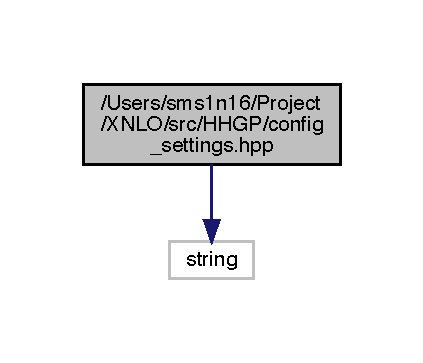
\includegraphics[width=203pt]{config__settings_8hpp__incl}
\end{center}
\end{figure}
This graph shows which files directly or indirectly include this file\+:\nopagebreak
\begin{figure}[H]
\begin{center}
\leavevmode
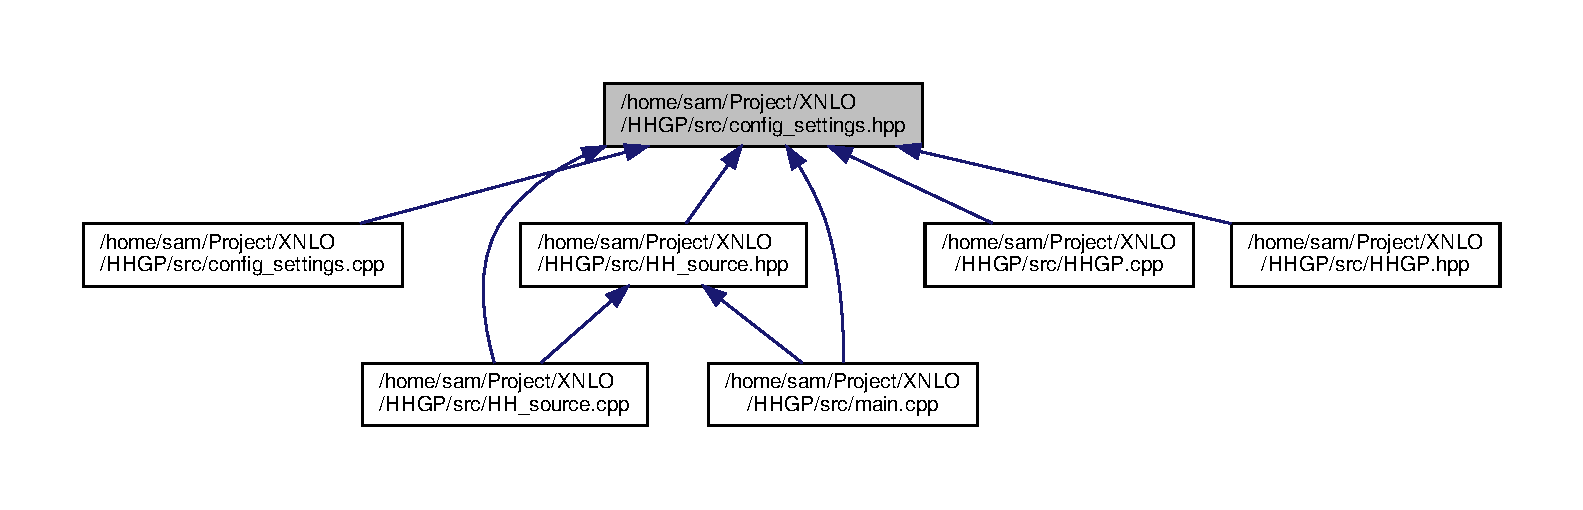
\includegraphics[width=350pt]{config__settings_8hpp__dep__incl}
\end{center}
\end{figure}
\subsection*{Classes}
\begin{DoxyCompactItemize}
\item 
class \hyperlink{class_config___settings}{Config\+\_\+\+Settings}
\end{DoxyCompactItemize}

\hypertarget{_h_h__source_8cpp}{}\section{/home/sam/\+Project/\+X\+N\+L\+O/\+H\+H\+G\+P/src/\+H\+H\+\_\+source.cpp File Reference}
\label{_h_h__source_8cpp}\index{/home/sam/\+Project/\+X\+N\+L\+O/\+H\+H\+G\+P/src/\+H\+H\+\_\+source.\+cpp@{/home/sam/\+Project/\+X\+N\+L\+O/\+H\+H\+G\+P/src/\+H\+H\+\_\+source.\+cpp}}
{\ttfamily \#include $<$iostream$>$}\newline
{\ttfamily \#include $<$string$>$}\newline
{\ttfamily \#include \char`\"{}Eigen/\+Dense\char`\"{}}\newline
{\ttfamily \#include \char`\"{}H\+H\+\_\+source.\+hpp\char`\"{}}\newline
{\ttfamily \#include \char`\"{}../../src/\+I\+O.\+hpp\char`\"{}}\newline
{\ttfamily \#include \char`\"{}config\+\_\+settings.\+hpp\char`\"{}}\newline
{\ttfamily \#include \char`\"{}../../src/maths\+\_\+textbook.\+hpp\char`\"{}}\newline
{\ttfamily \#include \char`\"{}../../src/\+D\+H\+T.\+hpp\char`\"{}}\newline

\hypertarget{_h_h__source_8hpp}{}\section{/home/sam/\+Project/\+X\+N\+L\+O/src/\+H\+H\+G\+P/\+H\+H\+\_\+source.hpp File Reference}
\label{_h_h__source_8hpp}\index{/home/sam/Project/XNLO/src/HHGP/HH\_source.hpp@{/home/sam/Project/XNLO/src/HHGP/HH\_source.hpp}}
{\ttfamily \#include $<$iostream$>$}\newline
{\ttfamily \#include $<$string$>$}\newline
{\ttfamily \#include \char`\"{}../../\+Eigen/\+Dense\char`\"{}}\newline
{\ttfamily \#include \char`\"{}../\+I\+O/\+I\+O.\+hpp\char`\"{}}\newline
{\ttfamily \#include \char`\"{}config\+\_\+settings.\+hpp\char`\"{}}\newline
{\ttfamily \#include \char`\"{}../maths/maths\+\_\+textbook.\+hpp\char`\"{}}\newline
{\ttfamily \#include \char`\"{}../\+D\+H\+T/\+D\+H\+T.\+hpp\char`\"{}}\newline
Include dependency graph for H\+H\+\_\+source.\+hpp\+:
\nopagebreak
\begin{figure}[H]
\begin{center}
\leavevmode
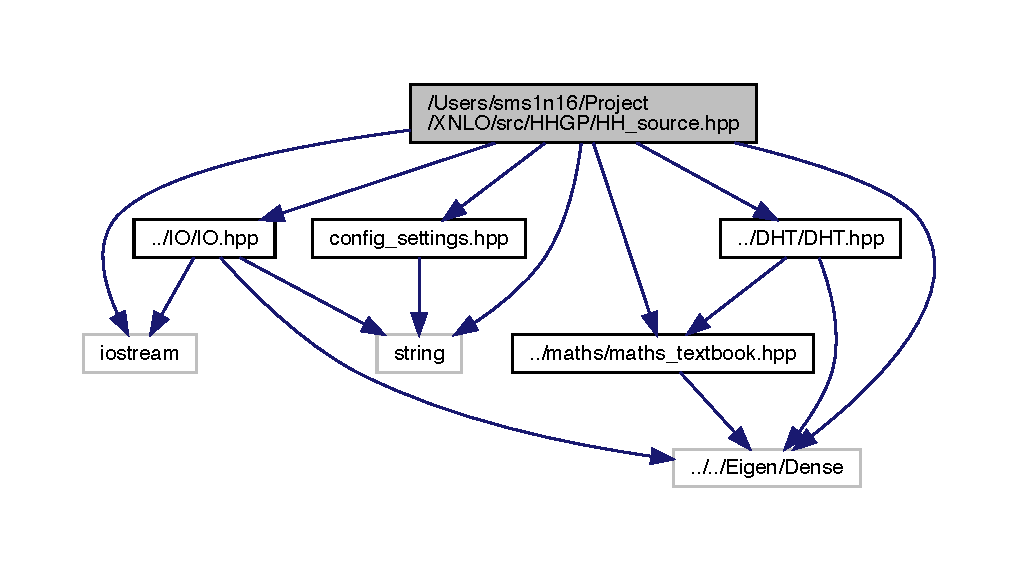
\includegraphics[width=350pt]{_h_h__source_8hpp__incl}
\end{center}
\end{figure}
This graph shows which files directly or indirectly include this file\+:
\nopagebreak
\begin{figure}[H]
\begin{center}
\leavevmode
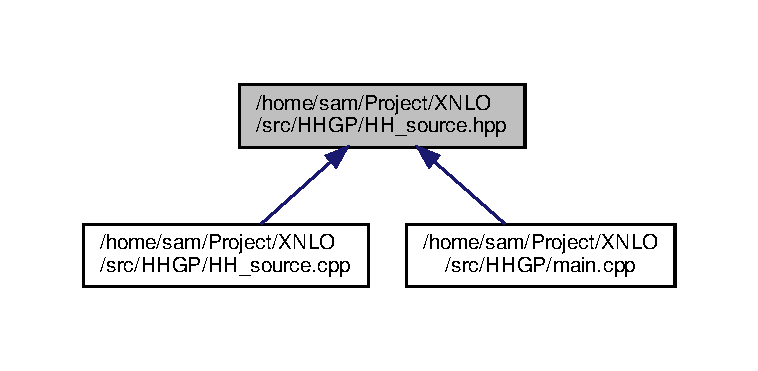
\includegraphics[width=350pt]{_h_h__source_8hpp__dep__incl}
\end{center}
\end{figure}
\subsection*{Classes}
\begin{DoxyCompactItemize}
\item 
class \mbox{\hyperlink{class_h_h__source}{H\+H\+\_\+source}}
\end{DoxyCompactItemize}

\hypertarget{_h_h_g_p_8cpp}{}\section{/home/sam/\+Project/\+X\+N\+L\+O/\+H\+H\+G\+P/src/\+H\+H\+GP.cpp File Reference}
\label{_h_h_g_p_8cpp}\index{/home/sam/\+Project/\+X\+N\+L\+O/\+H\+H\+G\+P/src/\+H\+H\+G\+P.\+cpp@{/home/sam/\+Project/\+X\+N\+L\+O/\+H\+H\+G\+P/src/\+H\+H\+G\+P.\+cpp}}
{\ttfamily \#include $<$iostream$>$}\newline
{\ttfamily \#include $<$string$>$}\newline
{\ttfamily \#include \char`\"{}../../\+Eigen/\+Dense\char`\"{}}\newline
{\ttfamily \#include \char`\"{}H\+H\+G\+P.\+hpp\char`\"{}}\newline
{\ttfamily \#include \char`\"{}config\+\_\+settings.\+hpp\char`\"{}}\newline
{\ttfamily \#include \char`\"{}../../src/maths\+\_\+textbook.\+hpp\char`\"{}}\newline
{\ttfamily \#include \char`\"{}../../src/keldysh\+\_\+gas.\+hpp\char`\"{}}\newline
{\ttfamily \#include \char`\"{}../../src/\+D\+H\+T.\+hpp\char`\"{}}\newline
{\ttfamily \#include \char`\"{}../../src/grid\+\_\+rkr.\+hpp\char`\"{}}\newline
{\ttfamily \#include \char`\"{}propagation.\+hpp\char`\"{}}\newline
{\ttfamily \#include \char`\"{}../../src/\+I\+O.\+hpp\char`\"{}}\newline
Include dependency graph for H\+H\+G\+P.\+cpp\+:
\nopagebreak
\begin{figure}[H]
\begin{center}
\leavevmode
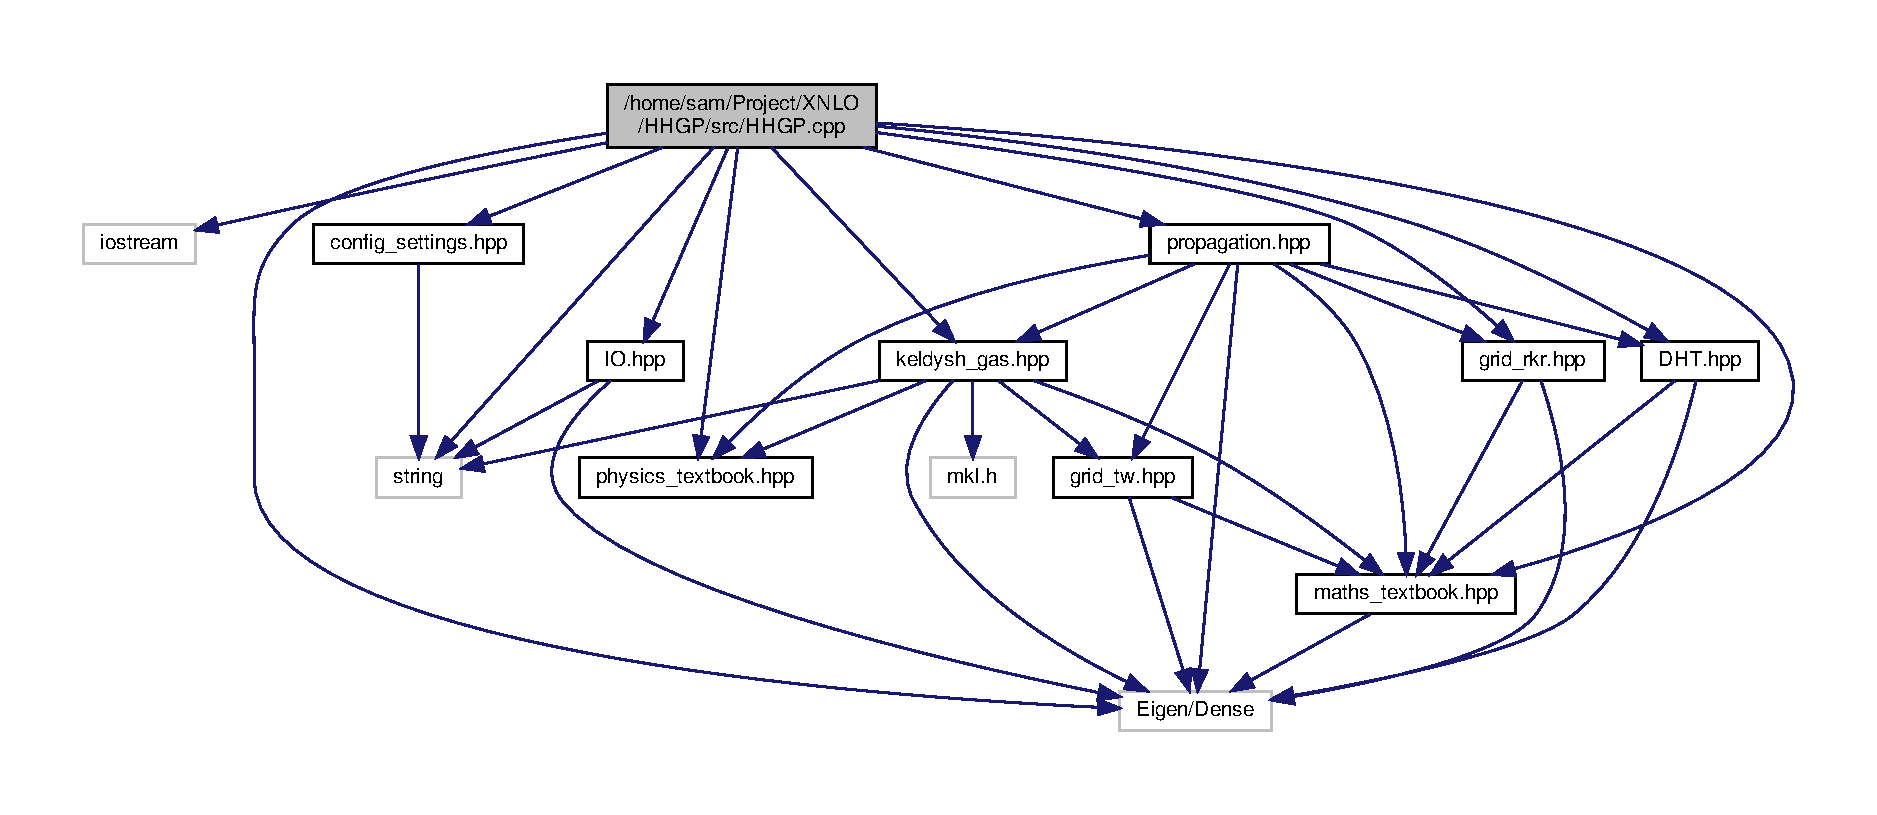
\includegraphics[width=350pt]{_h_h_g_p_8cpp__incl}
\end{center}
\end{figure}

\hypertarget{_h_h_g_p_8hpp}{}\section{/home/sam/\+Project/\+X\+N\+L\+O/src/\+H\+H\+G\+P/\+H\+H\+GP.hpp File Reference}
\label{_h_h_g_p_8hpp}\index{/home/sam/\+Project/\+X\+N\+L\+O/src/\+H\+H\+G\+P/\+H\+H\+G\+P.\+hpp@{/home/sam/\+Project/\+X\+N\+L\+O/src/\+H\+H\+G\+P/\+H\+H\+G\+P.\+hpp}}
{\ttfamily \#include \char`\"{}../../\+Eigen/\+Dense\char`\"{}}\newline
{\ttfamily \#include \char`\"{}config\+\_\+settings.\+hpp\char`\"{}}\newline
{\ttfamily \#include \char`\"{}../maths/maths\+\_\+textbook.\+hpp\char`\"{}}\newline
{\ttfamily \#include \char`\"{}../physics/physics\+\_\+textbook.\+hpp\char`\"{}}\newline
{\ttfamily \#include \char`\"{}../gas/keldysh\+\_\+gas.\+hpp\char`\"{}}\newline
{\ttfamily \#include \char`\"{}../\+D\+H\+T/\+D\+H\+T.\+hpp\char`\"{}}\newline
{\ttfamily \#include \char`\"{}../grid/grid\+\_\+rkr.\+hpp\char`\"{}}\newline
{\ttfamily \#include \char`\"{}propagation.\+hpp\char`\"{}}\newline
{\ttfamily \#include \char`\"{}../\+I\+O/\+I\+O.\+hpp\char`\"{}}\newline
Include dependency graph for H\+H\+G\+P.\+hpp\+:\nopagebreak
\begin{figure}[H]
\begin{center}
\leavevmode
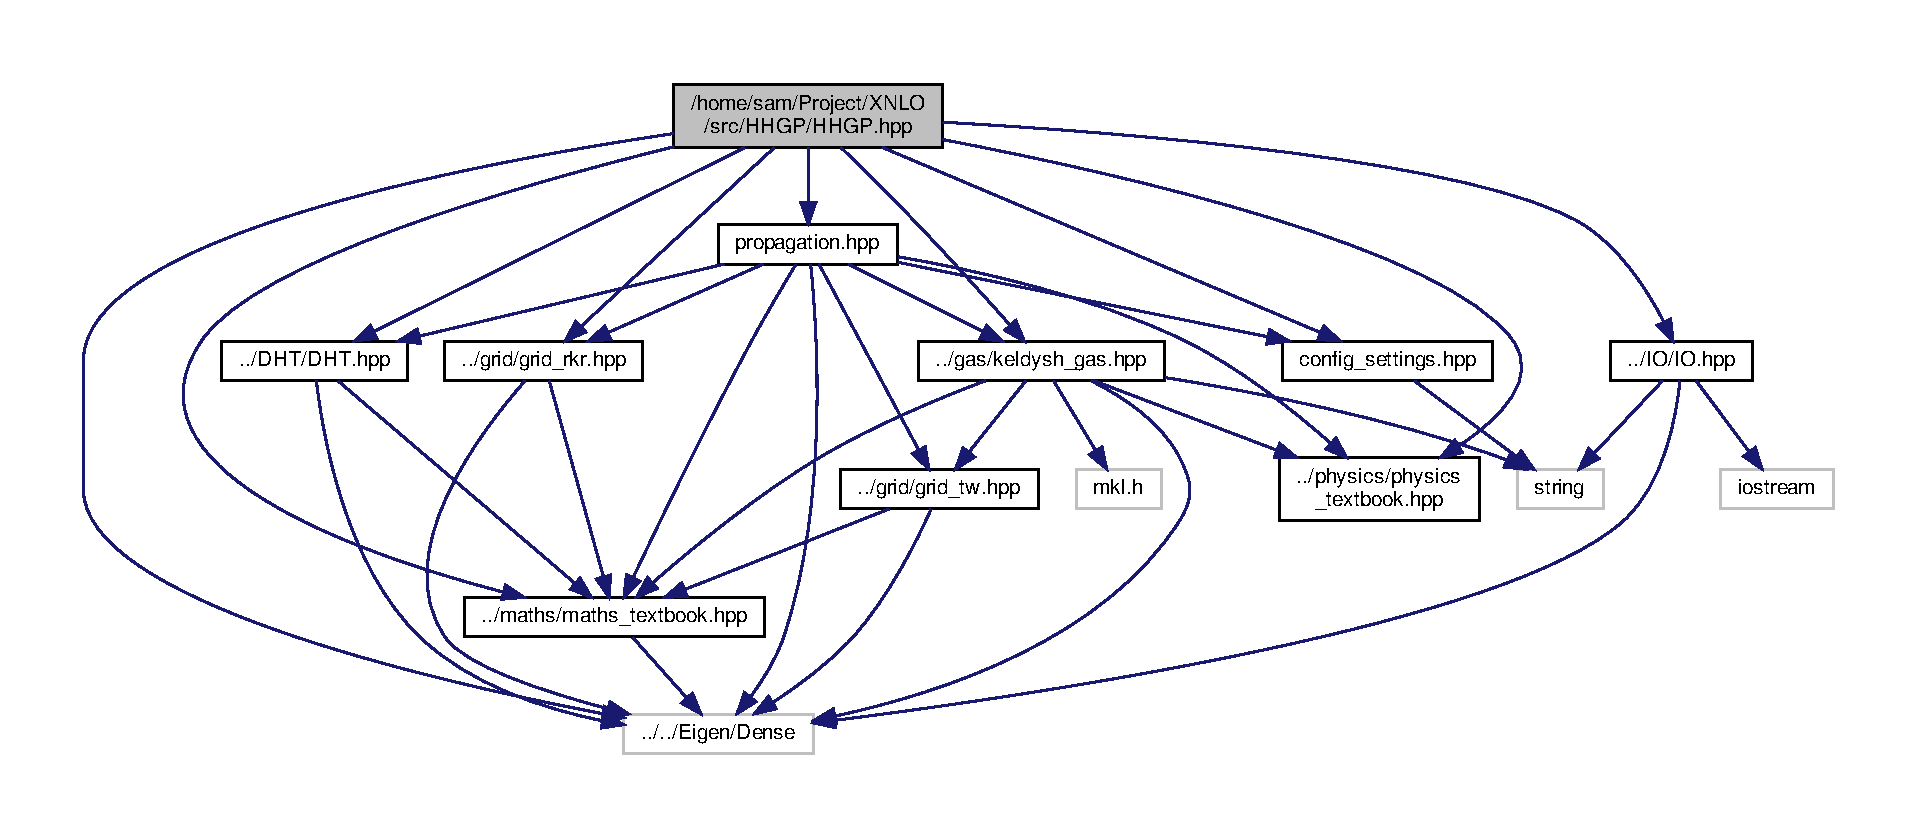
\includegraphics[width=350pt]{_h_h_g_p_8hpp__incl}
\end{center}
\end{figure}
This graph shows which files directly or indirectly include this file\+:\nopagebreak
\begin{figure}[H]
\begin{center}
\leavevmode
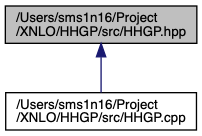
\includegraphics[width=209pt]{_h_h_g_p_8hpp__dep__incl}
\end{center}
\end{figure}
\subsection*{Classes}
\begin{DoxyCompactItemize}
\item 
class \hyperlink{class_h_h_g_p}{H\+H\+GP}
\end{DoxyCompactItemize}

\hypertarget{main_8cpp}{}\section{/home/sam/\+Project/\+X\+N\+L\+O/src/\+H\+H\+G\+P/main.cpp File Reference}
\label{main_8cpp}\index{/home/sam/Project/XNLO/src/HHGP/main.cpp@{/home/sam/Project/XNLO/src/HHGP/main.cpp}}
{\ttfamily \#include $<$iostream$>$}\newline
{\ttfamily \#include $<$string$>$}\newline
{\ttfamily \#include \char`\"{}../../\+Eigen/\+Dense\char`\"{}}\newline
{\ttfamily \#include \char`\"{}config\+\_\+settings.\+hpp\char`\"{}}\newline
{\ttfamily \#include \char`\"{}../maths/maths\+\_\+textbook.\+hpp\char`\"{}}\newline
{\ttfamily \#include \char`\"{}../physics/physics\+\_\+textbook.\+hpp\char`\"{}}\newline
{\ttfamily \#include \char`\"{}H\+H\+\_\+source.\+hpp\char`\"{}}\newline
{\ttfamily \#include \char`\"{}../gas/keldysh\+\_\+gas.\+hpp\char`\"{}}\newline
{\ttfamily \#include \char`\"{}../\+D\+H\+T/\+D\+H\+T.\+hpp\char`\"{}}\newline
{\ttfamily \#include \char`\"{}../grid/grid\+\_\+rkr.\+hpp\char`\"{}}\newline
{\ttfamily \#include \char`\"{}propagation.\+hpp\char`\"{}}\newline
{\ttfamily \#include \char`\"{}../\+I\+O/\+I\+O.\+hpp\char`\"{}}\newline
Include dependency graph for main.\+cpp\+:\nopagebreak
\begin{figure}[H]
\begin{center}
\leavevmode
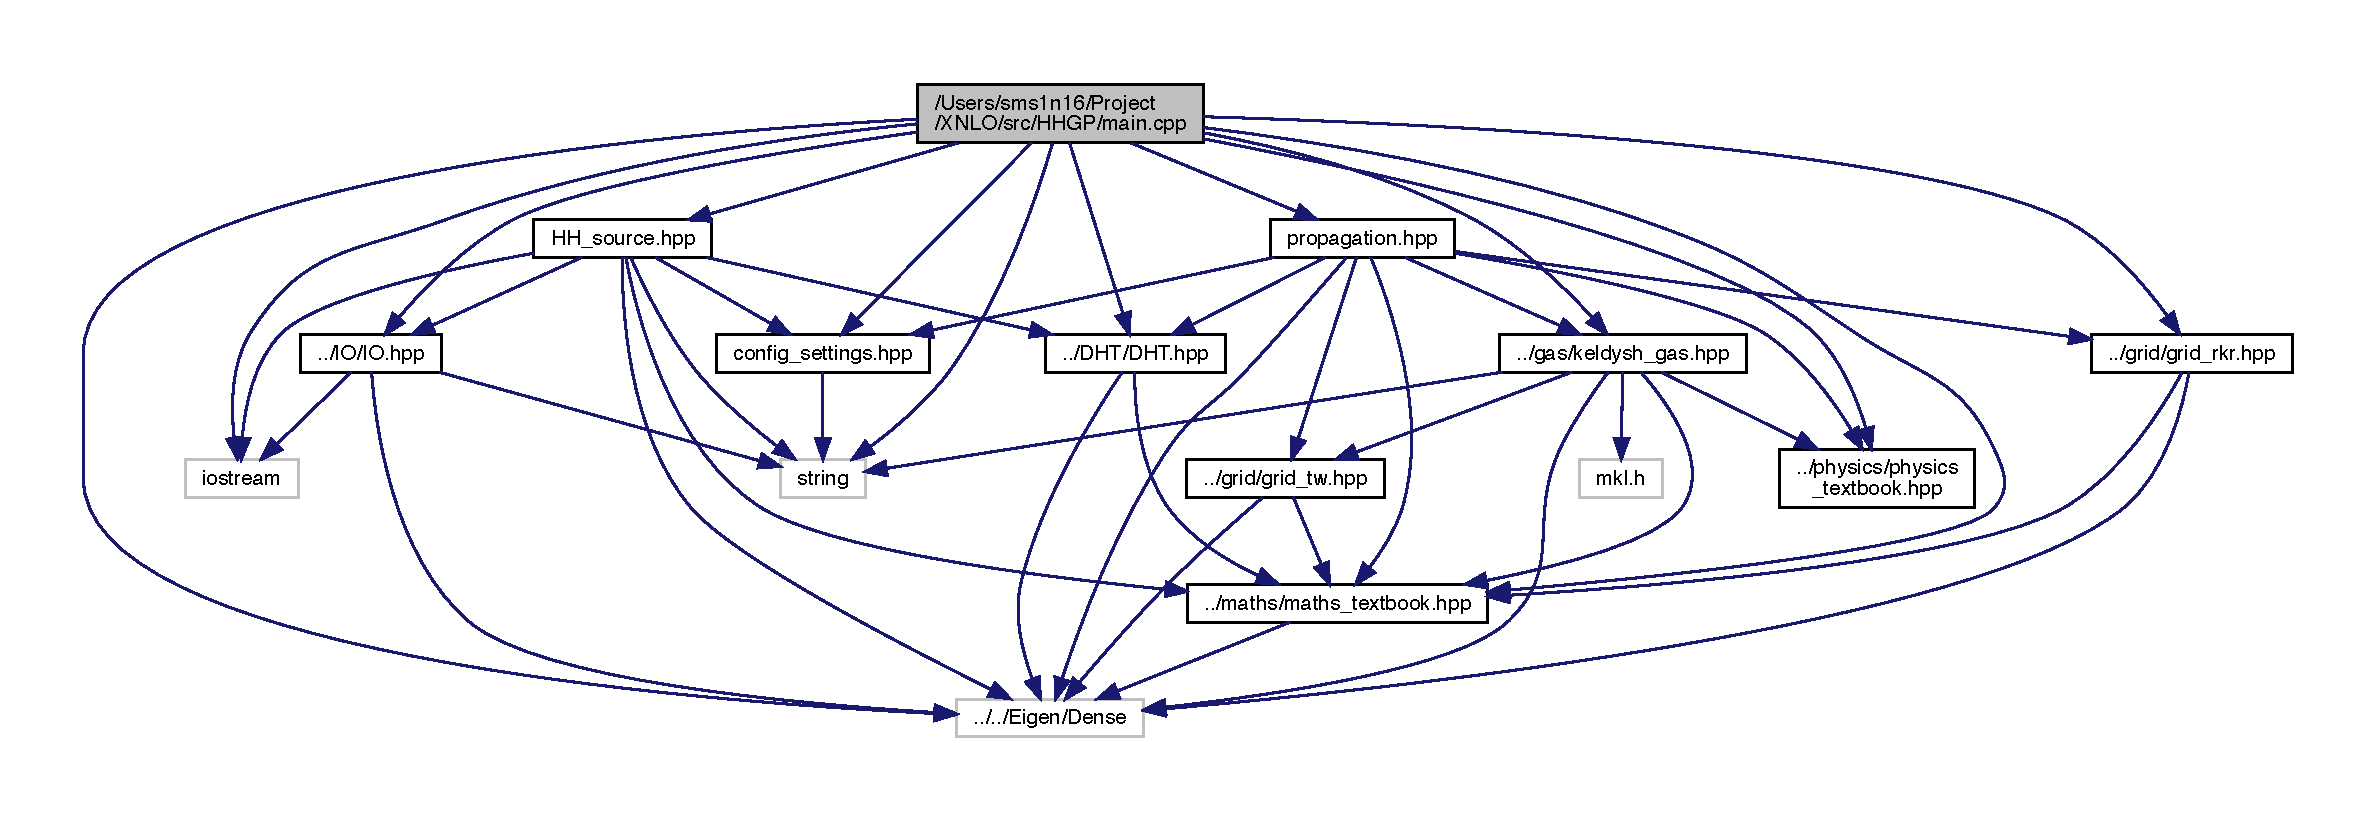
\includegraphics[width=350pt]{main_8cpp__incl}
\end{center}
\end{figure}
\subsection*{Functions}
\begin{DoxyCompactItemize}
\item 
int \mbox{\hyperlink{main_8cpp_a3c04138a5bfe5d72780bb7e82a18e627}{main}} (int argc, char $\ast$$\ast$argv)
\end{DoxyCompactItemize}


\subsection{Function Documentation}
\mbox{\Hypertarget{main_8cpp_a3c04138a5bfe5d72780bb7e82a18e627}\label{main_8cpp_a3c04138a5bfe5d72780bb7e82a18e627}} 
\index{main.cpp@{main.cpp}!main@{main}}
\index{main@{main}!main.cpp@{main.cpp}}
\subsubsection{\texorpdfstring{main()}{main()}}
{\footnotesize\ttfamily int main (\begin{DoxyParamCaption}\item[{int}]{argc,  }\item[{char $\ast$$\ast$}]{argv }\end{DoxyParamCaption})}

2.\+0; 
\hypertarget{propagation_8cpp}{}\section{/home/sam/\+Project/\+X\+N\+L\+O/\+H\+H\+G\+P/src/propagation.cpp File Reference}
\label{propagation_8cpp}\index{/home/sam/\+Project/\+X\+N\+L\+O/\+H\+H\+G\+P/src/propagation.\+cpp@{/home/sam/\+Project/\+X\+N\+L\+O/\+H\+H\+G\+P/src/propagation.\+cpp}}
{\ttfamily \#include \char`\"{}propagation.\+hpp\char`\"{}}\newline
{\ttfamily \#include \char`\"{}../../src/keldysh\+\_\+gas.\+hpp\char`\"{}}\newline
{\ttfamily \#include \char`\"{}../../src/grid\+\_\+rkr.\+hpp\char`\"{}}\newline
{\ttfamily \#include \char`\"{}../../src/grid\+\_\+tw.\+hpp\char`\"{}}\newline
{\ttfamily \#include \char`\"{}../../src/\+D\+H\+T.\+hpp\char`\"{}}\newline
{\ttfamily \#include \char`\"{}../../src/physics\+\_\+textbook.\+hpp\char`\"{}}\newline
{\ttfamily \#include \char`\"{}../../src/maths\+\_\+textbook.\+hpp\char`\"{}}\newline
{\ttfamily \#include \char`\"{}Eigen/\+Dense\char`\"{}}\newline
{\ttfamily \#include $<$iostream$>$}\newline
{\ttfamily \#include \char`\"{}../../src/\+I\+O.\+hpp\char`\"{}}\newline
{\ttfamily \#include $<$complex$>$}\newline
Include dependency graph for propagation.\+cpp\+:
\nopagebreak
\begin{figure}[H]
\begin{center}
\leavevmode
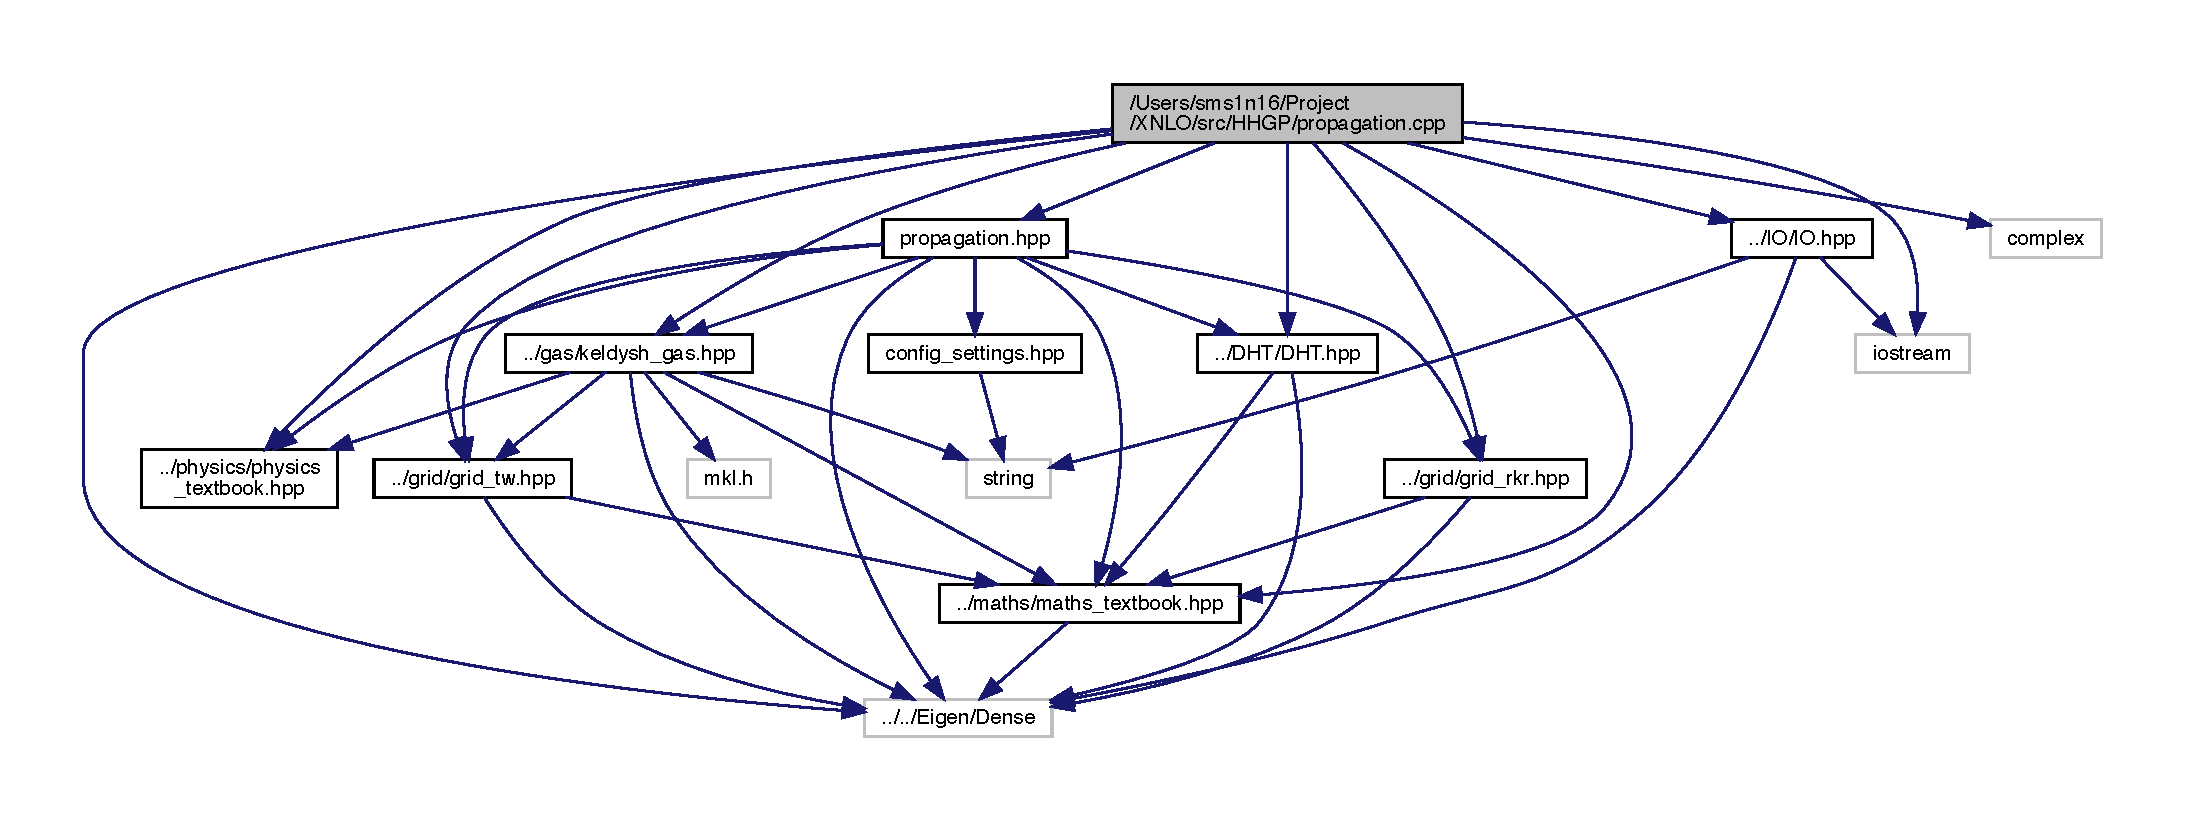
\includegraphics[width=350pt]{propagation_8cpp__incl}
\end{center}
\end{figure}

\hypertarget{propagation_8hpp}{}\section{/home/sam/\+Project/\+X\+N\+L\+O/src/\+H\+H\+G\+P/propagation.hpp File Reference}
\label{propagation_8hpp}\index{/home/sam/\+Project/\+X\+N\+L\+O/src/\+H\+H\+G\+P/propagation.\+hpp@{/home/sam/\+Project/\+X\+N\+L\+O/src/\+H\+H\+G\+P/propagation.\+hpp}}
{\ttfamily \#include \char`\"{}config\+\_\+settings.\+hpp\char`\"{}}\newline
{\ttfamily \#include \char`\"{}../gas/keldysh\+\_\+gas.\+hpp\char`\"{}}\newline
{\ttfamily \#include \char`\"{}../physics/physics\+\_\+textbook.\+hpp\char`\"{}}\newline
{\ttfamily \#include \char`\"{}../maths/maths\+\_\+textbook.\+hpp\char`\"{}}\newline
{\ttfamily \#include \char`\"{}../grid/grid\+\_\+rkr.\+hpp\char`\"{}}\newline
{\ttfamily \#include \char`\"{}../grid/grid\+\_\+tw.\+hpp\char`\"{}}\newline
{\ttfamily \#include \char`\"{}../\+D\+H\+T/\+D\+H\+T.\+hpp\char`\"{}}\newline
{\ttfamily \#include \char`\"{}../../\+Eigen/\+Dense\char`\"{}}\newline
Include dependency graph for propagation.\+hpp\+:\nopagebreak
\begin{figure}[H]
\begin{center}
\leavevmode
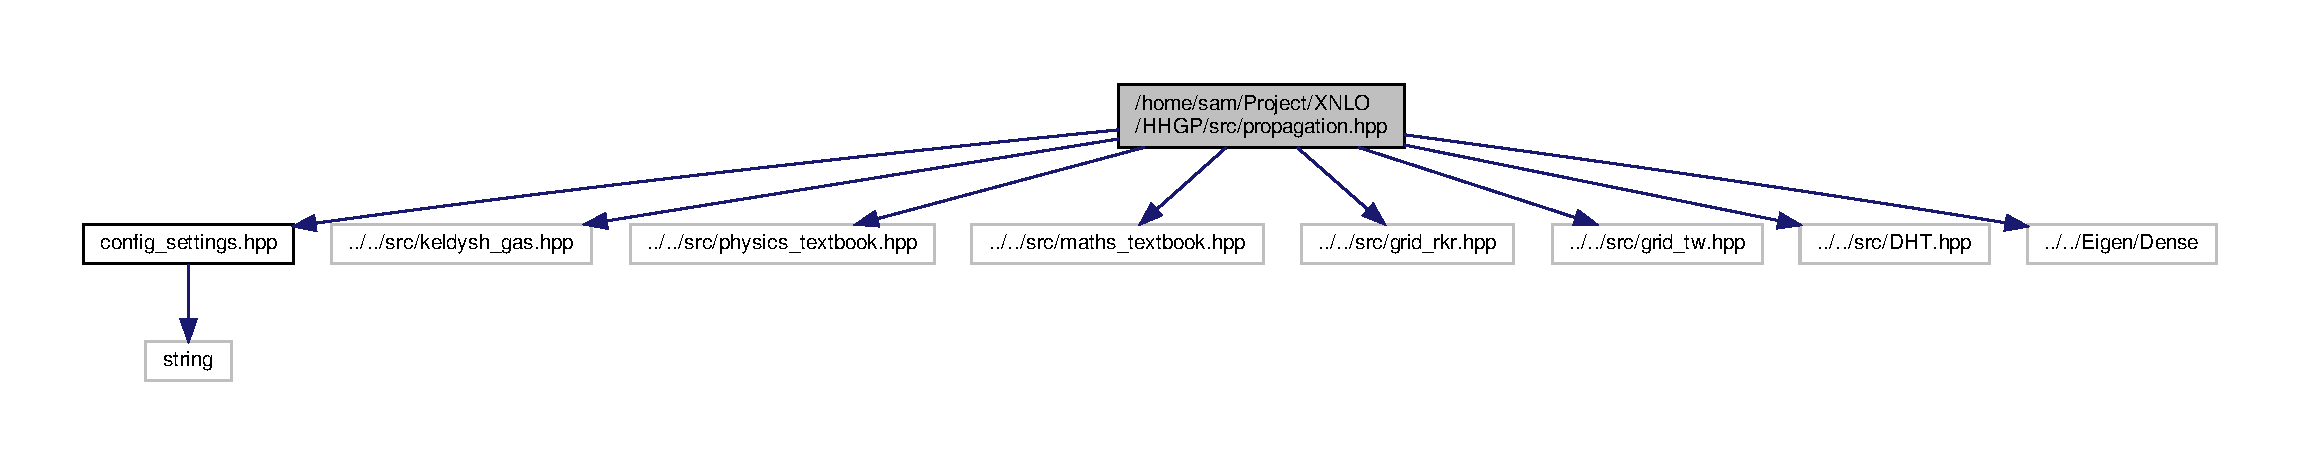
\includegraphics[width=350pt]{propagation_8hpp__incl}
\end{center}
\end{figure}
This graph shows which files directly or indirectly include this file\+:\nopagebreak
\begin{figure}[H]
\begin{center}
\leavevmode
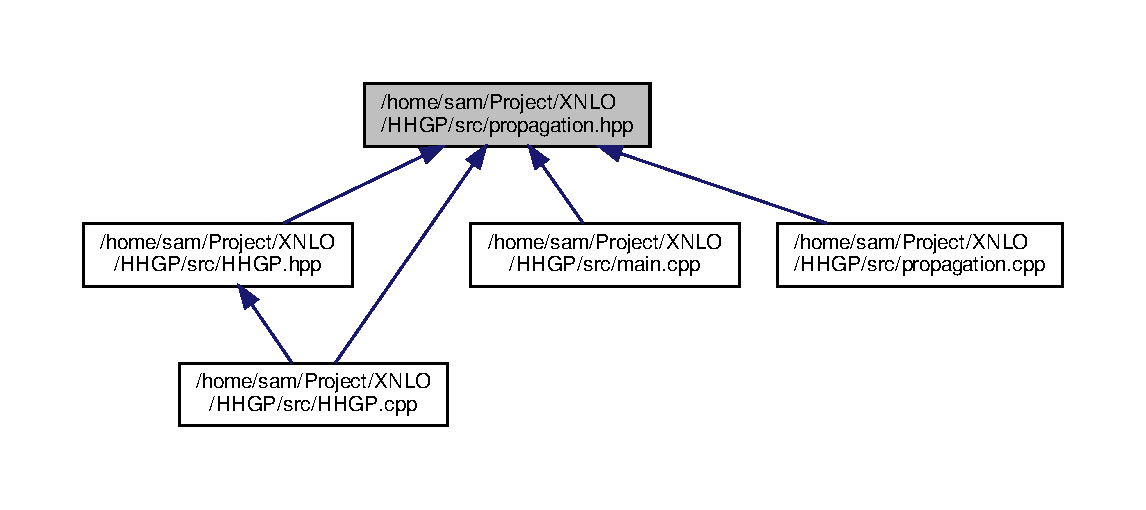
\includegraphics[width=350pt]{propagation_8hpp__dep__incl}
\end{center}
\end{figure}
\subsection*{Classes}
\begin{DoxyCompactItemize}
\item 
class \hyperlink{classpropagation}{propagation}
\end{DoxyCompactItemize}

\hypertarget{version_8hpp}{}\section{/home/sam/\+Project/\+X\+N\+L\+O/src/\+H\+H\+G\+P/version.hpp File Reference}
\label{version_8hpp}\index{/home/sam/\+Project/\+X\+N\+L\+O/src/\+H\+H\+G\+P/version.\+hpp@{/home/sam/\+Project/\+X\+N\+L\+O/src/\+H\+H\+G\+P/version.\+hpp}}
\subsection*{Macros}
\begin{DoxyCompactItemize}
\item 
\#define \hyperlink{version_8hpp_aac52b05128da45201ff8e39e39156b82}{\+\_\+\+V\+E\+R\+S\+I\+O\+N\+\_\+\+M\+A\+J\+OR}~2
\item 
\#define \hyperlink{version_8hpp_a1aac9829b460d4b1a2c8643fe7201524}{\+\_\+\+V\+E\+R\+S\+I\+O\+N\+\_\+\+M\+I\+N\+OR}~0
\item 
\#define \hyperlink{version_8hpp_abe78003459809bdd8d99f3b0b293b83f}{\+\_\+\+V\+E\+R\+S\+I\+O\+N\+\_\+\+S\+U\+B\+M\+I\+N\+OR}~0
\end{DoxyCompactItemize}


\subsection{Macro Definition Documentation}
\mbox{\Hypertarget{version_8hpp_aac52b05128da45201ff8e39e39156b82}\label{version_8hpp_aac52b05128da45201ff8e39e39156b82}} 
\index{version.\+hpp@{version.\+hpp}!\+\_\+\+V\+E\+R\+S\+I\+O\+N\+\_\+\+M\+A\+J\+OR@{\+\_\+\+V\+E\+R\+S\+I\+O\+N\+\_\+\+M\+A\+J\+OR}}
\index{\+\_\+\+V\+E\+R\+S\+I\+O\+N\+\_\+\+M\+A\+J\+OR@{\+\_\+\+V\+E\+R\+S\+I\+O\+N\+\_\+\+M\+A\+J\+OR}!version.\+hpp@{version.\+hpp}}
\subsubsection{\texorpdfstring{\+\_\+\+V\+E\+R\+S\+I\+O\+N\+\_\+\+M\+A\+J\+OR}{\_VERSION\_MAJOR}}
{\footnotesize\ttfamily \#define \+\_\+\+V\+E\+R\+S\+I\+O\+N\+\_\+\+M\+A\+J\+OR~2}

\mbox{\Hypertarget{version_8hpp_a1aac9829b460d4b1a2c8643fe7201524}\label{version_8hpp_a1aac9829b460d4b1a2c8643fe7201524}} 
\index{version.\+hpp@{version.\+hpp}!\+\_\+\+V\+E\+R\+S\+I\+O\+N\+\_\+\+M\+I\+N\+OR@{\+\_\+\+V\+E\+R\+S\+I\+O\+N\+\_\+\+M\+I\+N\+OR}}
\index{\+\_\+\+V\+E\+R\+S\+I\+O\+N\+\_\+\+M\+I\+N\+OR@{\+\_\+\+V\+E\+R\+S\+I\+O\+N\+\_\+\+M\+I\+N\+OR}!version.\+hpp@{version.\+hpp}}
\subsubsection{\texorpdfstring{\+\_\+\+V\+E\+R\+S\+I\+O\+N\+\_\+\+M\+I\+N\+OR}{\_VERSION\_MINOR}}
{\footnotesize\ttfamily \#define \+\_\+\+V\+E\+R\+S\+I\+O\+N\+\_\+\+M\+I\+N\+OR~0}

\mbox{\Hypertarget{version_8hpp_abe78003459809bdd8d99f3b0b293b83f}\label{version_8hpp_abe78003459809bdd8d99f3b0b293b83f}} 
\index{version.\+hpp@{version.\+hpp}!\+\_\+\+V\+E\+R\+S\+I\+O\+N\+\_\+\+S\+U\+B\+M\+I\+N\+OR@{\+\_\+\+V\+E\+R\+S\+I\+O\+N\+\_\+\+S\+U\+B\+M\+I\+N\+OR}}
\index{\+\_\+\+V\+E\+R\+S\+I\+O\+N\+\_\+\+S\+U\+B\+M\+I\+N\+OR@{\+\_\+\+V\+E\+R\+S\+I\+O\+N\+\_\+\+S\+U\+B\+M\+I\+N\+OR}!version.\+hpp@{version.\+hpp}}
\subsubsection{\texorpdfstring{\+\_\+\+V\+E\+R\+S\+I\+O\+N\+\_\+\+S\+U\+B\+M\+I\+N\+OR}{\_VERSION\_SUBMINOR}}
{\footnotesize\ttfamily \#define \+\_\+\+V\+E\+R\+S\+I\+O\+N\+\_\+\+S\+U\+B\+M\+I\+N\+OR~0}


%--- End generated contents ---

% Index
\backmatter
\newpage
\phantomsection
\clearemptydoublepage
\addcontentsline{toc}{chapter}{Index}
\printindex

\end{document}
